\documentclass[journal]{IEEEtran}

\usepackage{amsmath,amssymb,bm}
\usepackage{booktabs,multirow}
\usepackage{graphicx}
\usepackage{microtype}
\usepackage{xcolor}
\usepackage{url}
\usepackage{tikz}
\usetikzlibrary{arrows.meta,positioning}
\usepackage[hidelinks]{hyperref}

% Replace this file by running tools/export_latex.py after real evaluation.
% Values are percentages.  Never replace TBD by unmeasured estimates.
\newcommand{\MainPixelFOneFixed}{TBD}
\newcommand{\MainPixelIouFixed}{TBD}
\newcommand{\MainPixelAuc}{TBD}
\newcommand{\MainImageAuc}{TBD}
\newcommand{\MainPristinePixelFpr}{TBD}
\newcommand{\ResultSummary}{Quantitative results will be inserted after the preregistered evaluation is complete.}

\newcommand{\TBD}{\textcolor{red!70!black}{TBD}}
\newcommand{\method}{ReTraceNet}
\newcommand{\etal}{\textit{et al.}}
\newcommand{\R}{\mathbb{R}}

\title{ReTrace: Counterfactual Evidence Accounting for Faint Image Manipulation Localization}

\author{Anonymous Authors%
\thanks{Manuscript prepared for double-blind review. Replace this block with author affiliations only after the review policy permits.}}

\begin{document}
\maketitle

\begin{abstract}
Local image manipulation increasingly preserves semantic plausibility while
leaving only weak, spatially sparse traces. Existing localizers can correlate
such traces with a mask, but a high response does not establish that the trace---
rather than scene content or a dataset shortcut---caused the decision. We
introduce \method, a passive localization framework that tests forensic evidence
through an intra-image counterfactual intervention. A quality-conditioned
residual encoder first calibrates trace features and estimates their scale-wise
reliability. A candidate proposer then softly replaces suspicious trace tokens
with local/global pristine estimates from low-suspicion pixels of the same image,
while leaving the RGB content pathway unchanged. Factual and counterfactual
pyramids pass through strictly shared weights; their logit drop provides a
controlled measure of trace-specific effect. A dual-hypothesis evidence ledger
accumulates manipulation support and pristine counter-evidence across scales
instead of collapsing contradiction by feature fusion. Ledger conflict directly
conditions boundary refinement and predictive variance. Training combines
area-balanced heteroscedastic localization with counterfactual ranking, background
stability, ledger supervision, intervention locality, and causal-effect transport
consistency. The evaluation protocol spans classical and generative edits,
cross-dataset transfer, post-processing, pristine false alarms, and counterfactual
validity. \ResultSummary Code and configurations expose every intervention and
ledger component for controlled ablation.
\end{abstract}

\begin{IEEEkeywords}
Image forensics, manipulation localization, weak traces, counterfactual
intervention, evidence accounting, uncertainty estimation.
\end{IEEEkeywords}

\section{Introduction}
\IEEEPARstart{M}{odern} editing systems can remove, copy, splice, or regenerate a
small region without introducing an obvious semantic error.  The remaining clues
often lie in demosaicing noise, resampling correlations, local compression
history, or a narrow blending boundary.  These clues occupy different spatial
scales and are far weaker than the depicted content.  Image manipulation
localization (IML) must therefore solve a particularly unfavorable segmentation
problem: its most predictive training shortcuts are often the least transferable
forensic cues.

Existing approaches combine RGB with noise or frequency streams
\cite{zhou2018learning,wu2019mantranet,kwon2021catnet,guillaro2023trufor}, supervise
edges \cite{chen2021mvss,li2023edge}, or model long-range consistency
\cite{wang2022objectformer,guo2023hifi}. More recent designs add adaptive DCT and
content disentanglement \cite{wong2025adcd}, multi-spectral attention
\cite{nam2025m2sformer}, diffusion traces \cite{yu2024diffforensics}, or an ordered
sequence of masks for composite edits \cite{zhu2026rita}. These advances expose
complementary evidence, but they leave a different question open: would the
prediction change if the suspected forensic trace were absent while image content
remained fixed?

This question matters because correlation is not evidence attribution. A local
response may arise from a genuine acquisition inconsistency, an object boundary,
texture complexity, or dataset construction bias. Feature disentanglement can
reduce leakage, but it does not test whether the retained trace is necessary for
the decision. Ordinary augmentation changes both foreground and background,
whereas prototype matching measures similarity without observing a prediction
under intervention. Moreover, conventional multi-scale fusion compresses
supporting and contradicting observations into one latent tensor: weak agreement
and strong disagreement can become indistinguishable.

We address these gaps with \method. Given image $\mathbf{x}$, the network emits a
pixel mask, a log-variance map, and an image-level manipulation score:
\begin{equation}
(\mathbf{z},\mathbf{u},s)=F_{\theta}(\mathbf{x}),\qquad
\hat{\mathbf y}=\sigma(\mathbf z),
\label{eq:problem}
\end{equation}
where $\mathbf{x}\in[0,1]^{3\times H\times W}$, $\mathbf{u}$ measures predictive
ambiguity, and $s$ supports pristine-image screening.  Fig.~\ref{fig:overview}
summarizes the pipeline.

The method follows one causal chain and contains four separately falsifiable
technical contributions:
\begin{itemize}
\item We formulate passive IML as trace-specific counterfactual verification and
introduce intra-image counterfactual trace intervention (ICTI). It changes only
candidate trace tokens, derives replacement statistics from the same image, and
uses a strictly shared verifier to control branch capacity.
\item We propose a dual-hypothesis evidence ledger (DHEL) that writes non-negative
manipulation support and pristine counter-evidence at every scale. Quality-
conditioned reliability discounts each write, and bounded bidirectional transport
preserves contradiction that standard fusion would average away.
\item We derive conflict-guided boundary refinement (CBR) from the ledger. Its
uncertainty has a mechanistic component---simultaneous support and refutation---
and jointly controls boundary correction, heteroscedastic training, and image-
level pooling.
\item We develop objectives that prevent degenerate interventions: trace erasure
must lower logits inside manipulated regions, preserve background predictions,
remain spatially local, and transport the same causal effect across degradations.
\end{itemize}

\begin{figure*}[t]
\centering
\resizebox{0.98\textwidth}{!}{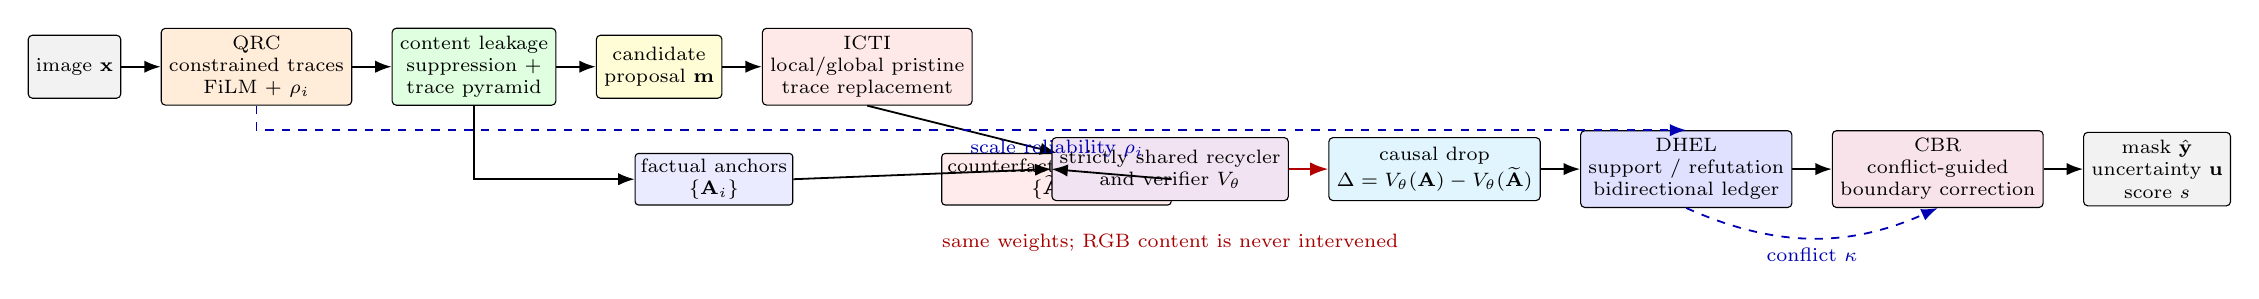
\begin{tikzpicture}[
  font=\scriptsize,
  node distance=4mm and 5mm,
  box/.style={draw, rounded corners=1.5pt, align=center, minimum height=8mm, inner sep=2.8pt},
  tinybox/.style={draw, rounded corners=1.2pt, align=center, minimum height=6.5mm, inner sep=2pt},
  flow/.style={-Latex, line width=0.65pt},
  causal/.style={-Latex, line width=0.8pt, color=red!70!black},
  evidence/.style={-Latex, dashed, line width=0.65pt, color=blue!70!black}
]
\node[box, fill=gray!10] (rgb) {image $\mathbf{x}$};
\node[box, fill=orange!15, right=of rgb] (qrc) {QRC\\constrained traces\\FiLM + $\rho_i$};
\node[box, fill=green!12, right=of qrc] (encoder) {content leakage\\suppression +\\trace pyramid};
\node[box, fill=yellow!16, right=of encoder] (proposal) {candidate\\proposal $\mathbf m$};
\node[box, fill=red!9, right=of proposal, minimum width=25mm] (icti) {ICTI\\local/global pristine\\trace replacement};

\node[tinybox, fill=blue!8, below left=6mm and -4mm of icti] (factual) {factual anchors\\$\{\mathbf A_i\}$};
\node[tinybox, fill=red!8, below right=6mm and -4mm of icti] (counter) {counterfactual anchors\\$\{\widetilde{\mathbf A}_i\}$};
\node[box, fill=violet!11, right=10mm of icti, yshift=-13mm] (verifier) {strictly shared recycler\\and verifier $V_\theta$};
\node[box, fill=cyan!12, right=of verifier] (effect) {causal drop\\$\Delta=V_\theta(\mathbf A)-V_\theta(\widetilde{\mathbf A})$};
\node[box, fill=blue!12, right=of effect] (ledger) {DHEL\\support / refutation\\bidirectional ledger};
\node[box, fill=purple!11, right=of ledger] (cbr) {CBR\\conflict-guided\\boundary correction};
\node[box, fill=gray!10, right=of cbr] (out) {mask $\hat{\mathbf y}$\\uncertainty $\mathbf u$\\score $s$};

\draw[flow] (rgb) -- (qrc);
\draw[flow] (qrc) -- (encoder);
\draw[flow] (encoder) -- (proposal);
\draw[flow] (proposal) -- (icti);
\draw[flow] (encoder.south) |- (factual.west);
\draw[flow] (icti.south) -- (counter.north);
\draw[flow] (factual.east) -- (verifier.west);
\draw[flow] (counter.east) -- (verifier.west);
\draw[causal] (verifier) -- (effect);
\draw[evidence] (qrc.south) |- node[pos=.78, below] {scale reliability $\rho_i$} (ledger.north);
\draw[flow] (effect) -- (ledger);
\draw[flow] (ledger) -- (cbr);
\draw[flow] (cbr) -- (out);
\draw[evidence] (ledger.south) to[bend right=24] node[below] {conflict $\kappa$} (cbr.south);
\node[align=center, below=3mm of verifier, text=red!65!black] {same weights; RGB content is never intervened};
\end{tikzpicture}
}
\caption{Overview of \method. ICTI creates a content-matched counterfactual in
trace space. Strictly shared weights isolate its prediction effect; DHEL retains
support and counter-evidence, whose conflict guides CBR.}
\label{fig:overview}
\end{figure*}

\section{Related Work}
\subsection{Forensic Trace Representation}
Handcrafted high-pass residuals and camera-model traces suppress image content,
but may fail under an unseen processing chain.  Constrained convolution
\cite{bayar2018constrained}, Noiseprint \cite{cozzolino2020noiseprint}, and
ManTra-Net \cite{wu2019mantranet} learn more general residual statistics.
CAT-Net jointly reasons over RGB and DCT coefficients \cite{kwon2021catnet}, while
TruFor combines RGB and a learned noise-sensitive fingerprint and estimates a
reliability map \cite{guillaro2023trufor}. ADCD-Net adaptively discounts DCT cues
under block misalignment, disentangles document content, and builds a pristine
prototype \cite{wong2025adcd}. Our quality module instead assigns reliability to
evidence writes, while the pristine estimate is used only to construct a
counterfactual whose effect is measured by a shared verifier.

\subsection{Multi-Scale and Boundary Reasoning}
MVSS-Net jointly exploits noise and boundary views with multi-scale supervision
\cite{chen2021mvss}.  ObjectFormer models object-level consistency
\cite{wang2022objectformer}; NCL treats contour patches as non-mutually-exclusive
contrastive samples \cite{zhou2023ncl}; and edge-aware message passing preserves
boundary cues \cite{li2023edge}. Recent systems expand the setting to large-scale
modern manipulations \cite{qu2024modern}, dynamic frequency context
\cite{xiang2024scca}, diffusion priors \cite{yu2024diffforensics}, and multi-
spectral attention \cite{nam2025m2sformer}. These methods learn a fused
representation. DHEL is different in representation and purpose: it maintains
two non-negative evidence accounts and exposes their conflict before writing them
back to decoder features.

\subsection{Generalization and Reliability}
Cross-dataset evaluation is essential because training-set artifacts can dominate
IML models.  CFL-Net \cite{niloy2023cfl} and NCL \cite{zhou2023ncl} use contrastive
learning to separate authentic and manipulated distributions.  HiFi-Net exploits
hierarchical manipulation attributes \cite{guo2023hifi}; TrainFors highlights the
effect of nonstandardized training data \cite{nandi2023trainfors}.  Our protocol
therefore fixes training data, adds pristine images, discloses threshold selection,
and measures calibration under post-processing.

\subsection{Process Modeling and Counterfactual Verification}
RITA reformulates composite manipulation localization as autoregressive mask
prediction over editing steps \cite{zhu2026rita}; OmniGuard combines active
watermarking with passive extraction \cite{zhang2025omniguard}. Our setting is
passive and does not reconstruct an unknown edit sequence. ICTI asks a local
necessity question inside a single observed image: after replacing only the
suspected trace with an internally estimated pristine trace, does a weight-shared
detector withdraw its claim? This controlled factual/counterfactual comparison is
also distinct from augmentation consistency, which changes acquisition cues in
the entire image.

\begin{table*}[t]
\centering
\caption{Mechanism-level positioning relative to representative recent IML
designs. ``Intervention'' means changing candidate forensic features while
holding the content path and verifier weights fixed; it is stricter than using a
prototype as an additional feature.}
\label{tab:mechanism_position}
\setlength{\tabcolsep}{4.2pt}
\begin{tabular}{lccccc}
\toprule
Method & Quality/reliability use & Content or pristine modeling & Trace intervention
& Matched effect & Explicit support/refutation\\
\midrule
TruFor \cite{guillaro2023trufor} & output confidence & RGB/noise fusion & -- & -- & --\\
M2SFormer \cite{nam2025m2sformer} & -- & multi-spectral attention & -- & -- & --\\
ADCD-Net \cite{wong2025adcd} & adaptive DCT score & disentanglement + prototype & -- & -- & --\\
RITA \cite{zhu2026rita} & -- & ordered mask history & -- & -- & --\\
\method{} & scale write reliability & same-image pristine estimator & ICTI
& shared verifier drop & DHEL + conflict\\
\bottomrule
\end{tabular}
\end{table*}

\section{Method}
\subsection{Forensic Intervention Formulation}
\label{sec:formulation}

Our starting point is a distinction between \emph{predictive correlation} and
\emph{trace-specific evidence}. A pixel may receive a high manipulation score
because its residual is inconsistent with the rest of the image, but it may also
receive the same score because it belongs to a salient object boundary that is
over-represented in the training masks. Feature separation reduces the second
failure mode only indirectly. We instead ask whether a suspected trace is
necessary for the prediction. Let $\mathbf A=\{\mathbf A_i\}_{i=1}^L$ denote the
observed forensic pyramid and let $\mathcal I(\mathbf A,\mathbf m)$ replace traces
selected by proposal $\mathbf m$ without changing the RGB content path. We call
$\widetilde{\mathbf A}=\mathcal I(\mathbf A,\mathbf m)$ a trace counterfactual.
For a weight-shared verifier $V_\theta$, the pixel-wise effect is positive when
removing the trace withdraws manipulation evidence. This construction embodies
three controls: factual and counterfactual inputs come from the same image, their
content features are identical, and their verifier parameters are identical.

The proposal is necessarily imperfect. Hence, a single positive effect cannot be
treated as proof. \method{} maintains two hypotheses throughout decoding:
$H_1$ states that a local manipulation trace is present, whereas $H_0$ states that
the observed deviation is compatible with the pristine image. Every scale writes
support for both hypotheses. Their ratio yields a decision; their simultaneous
strength yields conflict. This causal-effect-and-ledger formulation determines
the order of all modules below: quality calibration must precede intervention,
intervention must precede evidence accounting, and ledger conflict must precede
uncertainty-guided refinement.

\textbf{Design principle and novelty boundary.}
The framework is deliberately not a collection of interchangeable attention
blocks. Its state changes have distinct meanings. QRC estimates whether a trace
observation is trustworthy; ICTI asks what the prediction would be without that
observation; the shared verifier measures the resulting withdrawal of evidence;
DHEL records support and refutation without cancelling either; and CBR spends
additional capacity where those accounts disagree. Removing an earlier stage
therefore changes the input semantics of every later stage. This ordering also
separates our objective from frequency selection, prototype matching, or generic
two-branch fusion: none of those operations by itself tests the necessity of a
suspected trace while preserving the content path and verifier. We use
``counterfactual'' in this operational, model-internal sense rather than claiming
to reconstruct the unknown unedited photograph. The intervention supplies a
controlled diagnostic contrast, and the ledger makes the limitations of that
contrast visible as conflict instead of converting it immediately into a hard
mask.

\subsection{Quality-Conditioned Trace Observation}
\label{sec:qrc}

\textbf{Exactly constrained residuals.}
The RGB path preserves scene structure, while the trace path begins with $M$
learnable $5\!\times\!5$ residual kernels. For the $m$th kernel and center
$p_0$, we impose
\begin{equation}
\sum_{c,p}\mathbf K_m(c,p)=0,\quad
\sum_c\mathbf K_m(c,p_0)=-1,\quad
\sum_{c,p\ne p_0}\mathbf K_m(c,p)=1.
\label{eq:new_constraint}
\end{equation}
The three center coefficients are $-1/3$; all non-center coefficients are a
softmax over unconstrained parameters. Equation~\eqref{eq:new_constraint} is
therefore satisfied on every forward pass rather than approximately restored
after optimization. The zero DC response suppresses locally constant appearance,
but it does not make residual strength comparable across unknown processing
chains.

\textbf{Calibration and evidential reliability.}
From grayscale image $g$, we measure mean, standard deviation, saturation ratio,
horizontal/vertical gradient energy, Laplacian energy, and nominal 8-pixel block
boundary energy:
\begin{equation}
\begin{split}
\mathbf q&=[\mu_g,\sigma_g,\rho_{\rm sat},E_x,E_y,E_{\rm lap},B_x,B_y],\\
\bar{\mathbf T}_i&=(1+0.5\tanh\bm\gamma_i)\odot\mathbf T_i
                  +0.5\tanh\bm\beta_i,\quad
\rho_i=\sigma(r_i),
\end{split}
\label{eq:new_quality}
\end{equation}
where $(\bm\gamma_i,\bm\beta_i,r_i)$ are produced by a small MLP from $\mathbf q$.
The FiLM terms calibrate the observation; scalar $\rho_i\in(0,1)$ states how much
the ledger should trust scale $i$. This division is important. A strongly
recompressed image can still contain a large high-frequency response, yet that
response should receive low evidential weight. The final MLP layer is initialized
to zero, making FiLM an identity and $\rho_i=0.5$ at the beginning of training.

\textbf{Content leakage suppression.}
QRC is followed by a lightweight safeguard rather than treated as a principal
contribution. Aligned trace and content vectors are locally projected:
\begin{equation}
\mathbf T_i^\perp=\bar{\mathbf T}_i-\sigma(a_i)
\frac{\langle\bar{\mathbf T}_i,\mathbf C_i\rangle}
{\|\mathbf C_i\|_2^2+\epsilon}\mathbf C_i,\qquad
\mathbf A_i=\operatorname{LN}(\mathbf W_i*\mathbf T_i^\perp).
\label{eq:new_orth_anchor}
\end{equation}
The projected and original traces are mixed before $\mathbf W_i$, so useful
content-coupled acquisition statistics are not irreversibly deleted. All anchors
have width $d$. We do not claim that orthogonality alone establishes forensic
causality; it merely reduces leakage before the explicit intervention test.

The distinction between calibration and reliability is also consequential for
optimization. If quality descriptors directly gated the final mask, the model
could learn dataset-specific correlations such as ``strong compression implies
tampering.'' Here they can only rescale trace observations and discount evidence
writes. A low $\rho_i$ cannot create pristine evidence, nor can it suppress the
RGB content path; it merely limits how strongly a questionable forensic scale
votes in DHEL. Conversely, FiLM cannot decide the final class because its output
must still survive intervention and shared verification. The two outputs of QRC
thus constrain one another: calibration improves observability, while reliability
prevents an amplified but unstable response from dominating the ledger. Per-scale
reliability further permits a blurred image to distrust the finest scale while
retaining useful block or region statistics at coarser scales.

\subsection{Intra-Image Counterfactual Trace Intervention}
\label{sec:icti}

ICTI constructs an alternative trace pyramid that is plausible under $H_0$ and
matched in semantic content. It contains a proposal, an image-internal pristine
estimator, and a soft intervention. No external generator or pristine reference
image is needed.

\textbf{Proposal and intervention curriculum.}
The finest anchor yields proposal logits $\mathbf a=P(\mathbf A_1)$ and candidate
probability $\mathbf m=\sigma(\mathbf a)$. During training, early proposals may
miss the entire manipulated region, in which case the counterfactual would equal
the factual input and provide no gradient. With probability $p_e=p_0\eta^e$ at
epoch $e$, we mix the resized ground-truth mask into the intervention selector:
\begin{equation}
\mathbf m_i^{(e)}=(1-\lambda_t)\mathcal R_i(\sigma(\mathbf a))
 +\lambda_t\mathcal R_i(\mathbf y),\qquad p_e=p_0\eta^e.
\label{eq:new_curriculum}
\end{equation}
We use $p_0=0.6$, $\eta=0.95$, and $\lambda_t=0.5$. When teacher forcing is not
sampled, the first term is used alone; inference never observes $\mathbf y$.
Proposal BCE and Dice supervision ensure that the selector remains meaningful
after the curriculum decays.

\textbf{Pristine trace estimation from the same image.}
Let $\mathbf b_i=1-\operatorname{sg}(\mathbf m_i)$ be detached background weights.
For pixel $p$, local and global pristine estimates are
\begin{equation}
\mathbf l_i(p)=
\frac{\sum_{q\in\mathcal N(p)}b_i(q)\mathbf A_i(q)}
     {\sum_{q\in\mathcal N(p)}b_i(q)+\epsilon},\qquad
\mathbf g_i=
\frac{\sum_q b_i(q)\mathbf A_i(q)}{\sum_q b_i(q)+\epsilon}.
\label{eq:new_pristine}
\end{equation}
The local estimate preserves spatially varying camera and compression statistics;
the global estimate is a stable fallback when $\mathcal N(p)$ is mostly
suspicious. Detaching $\mathbf b_i$ prevents the proposer from changing merely to
make pristine estimation easier. A gated convolution
$R_i=R([\mathbf A_i,\mathbf l_i,\mathbf g_i,\mathbf m_i])$ selects between the two
contexts and adapts them to the candidate location. The adapter is bounded to
$0.1\tanh(\cdot)$ around their convex mixture; it therefore corrects estimation
bias without becoming an unconstrained feature generator.

\textbf{Soft trace erasure.}
A learned gate $h_i\in(0,1)$ controls intervention strength. The counterfactual
anchor and observable intervention energy are
\begin{equation}
\widetilde{\mathbf A}_i=\mathbf A_i+\mathbf m_i h_i\odot
(\mathbf R_i-\mathbf A_i),\qquad
\mathbf e_i=\operatorname{mean}_c|\mathbf A_i-\widetilde{\mathbf A}_i|.
\label{eq:new_intervention}
\end{equation}
Hard replacement would create a new edge at the proposal boundary and allow the
detector to recognize its own intervention. The soft form makes replacement
continuous and exposes $\mathbf m_i h_i$ for a background-locality penalty. Since
only trace anchors are altered, both branches reuse the exact RGB content
features already absorbed during leakage suppression.

ICTI contains three safeguards against a trivial counterfactual. First, the
replacement is estimated only from the current image, so the branch cannot use
the identity of an external donor as an easy cue. Second, the selector is
supervised but detached when it defines pristine weights; otherwise it could
expand the presumed-pristine set solely to minimize reconstruction error. Third,
the residual adapter and intervention gate are bounded, while off-target energy
is penalized. An all-zero intervention is rejected by proposal supervision and
the positive-region ranking loss; an all-image intervention is rejected by
background stability and locality; an adversarial replacement is restricted by
the convex local/global estimate and bounded adapter. These controls do not prove
that $\widetilde{\mathbf A}_i$ is the true pristine feature. They make the learned
contrast falsifiable: a useful intervention must be localized, lower the factual
score within manipulated pixels, preserve background predictions, and remain
stable under benign degradation.

\subsection{Strictly Shared Causal Verification}
\label{sec:verifier}

The factual and counterfactual anchors are independently transported by the same
multi-scale operator. Starting from $\mathbf H_i^0=\mathbf A_i$ (or
$\widetilde{\mathbf A}_i$), each iteration re-injects its immutable anchor and
exchanges neighboring-scale context:
\begin{equation}
\begin{split}
\overleftarrow{\mathbf H}_i^k&=\Phi_{\rm td}(\mathbf H_i^{k-1},
\mathcal R(\overleftarrow{\mathbf H}_{i+1}^k),\mathbf H_i^0),\\
\mathbf H_i^k&=\Phi_{\rm bu}(\overleftarrow{\mathbf H}_i^k,
\mathcal R(\mathbf H_{i-1}^k),\mathbf H_i^0).
\end{split}
\label{eq:new_transport}
\end{equation}
$\Phi_{\rm td}$ and $\Phi_{\rm bu}$ are gated ConvNeXt-style cells shared across
scales and across the two branches. We use two iterations. The shared verifier
$V_\theta$ then produces factual and counterfactual logits. Their controlled
effect is
\begin{equation}
\Delta(p)=V_\theta(\{\mathbf H_i^K\})(p)-
V_\theta(\{\widetilde{\mathbf H}_i^K\})(p).
\label{eq:new_effect}
\end{equation}
Because the branches differ only through Eq.~\eqref{eq:new_intervention}, a
positive $\Delta$ is evidence that the erased trace supported the original
decision. Shared weights are essential: independent decoders could manufacture a
large $\Delta$ through parameter asymmetry. We inject only
$\operatorname{ReLU}(\Delta)$ into the final manipulation logit. Negative effects
are not discarded, however; they enter the refutation account below.

\subsection{Dual-Hypothesis Evidence Ledger}
\label{sec:dhel}

\textbf{Local evidence writes.}
At every scale, a shared writer compares the factual state, counterfactual state,
and their signed difference. Two softplus outputs create non-negative support
$s_i$ and refutation $r_i$:
\begin{equation}
[s_i,r_i]=\rho_i\operatorname{softplus}\!\left(
W_E*[\mathbf H_i^K,\widetilde{\mathbf H}_i^K,
\mathbf H_i^K-\widetilde{\mathbf H}_i^K]\right)+\epsilon.
\label{eq:new_write}
\end{equation}
The writer is not constrained to interpret every feature difference as support.
For example, a large difference that fails to lower the factual logit can be
written as refutation. Multiplication by $\rho_i$ connects acquisition quality to
evidential strength rather than to the final probability directly.

\textbf{Bounded bidirectional accounting.}
Let $\mathbf L_i=[s_i,r_i]$. Coarse-to-fine transport supplies region context;
fine-to-coarse transport returns boundary counter-evidence:
\begin{equation}
\overleftarrow{\mathbf L}_i=\mathbf L_i+\sigma(\alpha_i)
\mathcal R(\overleftarrow{\mathbf L}_{i+1}),\qquad
\mathbf L_i^*=\overleftarrow{\mathbf L}_i+\sigma(\beta_i)
\mathcal R(\mathbf L_{i-1}^*).
\label{eq:new_ledger_transport}
\end{equation}
The sigmoid-bounded discounts prevent one scale from contributing unbounded
evidence. Unlike feature addition, both ledger channels retain their identity
through transport. Consequently, a location with $(s,r)=(0.1,0.1)$ is distinct
from $(s,r)=(10,10)$ even though both have zero signed difference.

\textbf{Decision and conflict.}
For the aggregated support/refutation at each scale, we compute
\begin{equation}
\ell_i=\log(s_i^*+\epsilon)-\log(r_i^*+\epsilon),\qquad
\kappa_i=\frac{2\min(s_i^*,r_i^*)}{s_i^*+r_i^*+\epsilon}
\left(1-e^{-(s_i^*+r_i^*)}\right).
\label{eq:new_conflict}
\end{equation}
$\ell_i$ is a supervised manipulation log-odds; $\kappa_i\in[0,1]$ is high only
when both hypotheses have comparable and non-trivial strength. The exponential
mass factor prevents two negligible accounts from appearing maximally uncertain.
Five interpretable maps---normalized support, normalized refutation, conflict,
evidence mass, and intervention energy---are embedded and written back to the factual state. DHEL therefore retains an
auditable evidence representation while still providing rich decoder features.

This ledger differs from concatenating multi-scale features in two ways. First,
its channels have fixed hypothesis semantics at every resolution, so transport
cannot silently rotate support into refutation. Second, conflict depends on both
balance and evidence mass. Standard entropy is high for a probability near one
half even when the network has observed almost nothing; $\kappa_i$ instead becomes
large only when substantial evidence supports both hypotheses. This matters near
real splice boundaries, where an editing trace and a natural edge can coexist,
and in heavily compressed regions, where all accounts should remain weak. The
causal effect and intervention energy are included in the ledger writeback but do
not overwrite the accounts. DHEL can therefore express three different states:
confident manipulation, confident pristine content, and unresolved contradiction.
CBR consumes the third state explicitly rather than forcing DHEL to make a
premature binary decision.

\subsection{Conflict-Guided Boundary Refinement}
\label{sec:cbr}

The finest ledger-enriched state gives coarse logit $z^0$ and learned log-variance
$u^0$. Its probability gradient $b=\|\nabla\sigma(z^0)\|_2$ identifies a candidate
boundary. Learned uncertainty and ledger conflict are mixed, then supplied with
intervention energy to a residual head:
\begin{equation}
\begin{split}
q&=(1-\omega)\sigma(u^0)+\omega\kappa_1,
\quad \omega=\sigma(w),\\
(\delta z,\delta u)&=G([\mathbf H_1^{\rm led},\sigma(z^0),b,q,
\kappa_1,e_1]),\\
z&=z^0+(0.5+q)\delta z+\sigma(g)\operatorname{ReLU}(\Delta),
\quad u=\operatorname{logit}(q)+\delta u.
\end{split}
\label{eq:new_refine}
\end{equation}
This design makes uncertainty operational and partially mechanistic. High ledger
conflict expands the correction budget, whereas a strong RGB boundary with weak
intervention effect is not automatically amplified. The factual/counterfactual
effect is added only after their matched verification, preserving the controlled
contrast.

For image-level screening, reliability $c_p=\exp(-u_p)$ weights spatial evidence.
An MLP $h$ maps reliable mean and maximum to score $s$:
\begin{equation}
s=h\!\left(\frac{\sum_p c_p\sigma(z_p)}{\sum_p c_p+\epsilon},
\max_p c_p\sigma(z_p)\right).
\label{eq:new_image_score}
\end{equation}
Thus, ledger conflict affects both pixel refinement and the confidence assigned to
the whole-image decision.

\subsection{Non-Degenerate Causal Training}
\label{sec:loss}

\textbf{Localization and boundary terms.}
Small regions would otherwise be dominated by pristine pixels. With manipulated
area $A_+$ and background area $A_-$, define
$w_+=\operatorname{clip}(\sqrt{(A_-+1)/(A_++1)},1,w_{\max})$. The primary loss is
\begin{equation}
\mathcal L_{\rm het}=\frac1{HW}\sum_p w(y_p)e^{-u_p}
\operatorname{BCE}(z_p,y_p)+\tfrac12u_p,
\label{eq:new_hetero}
\end{equation}
combined with soft Dice and BCE between morphological gradients of prediction and
mask. Auxiliary decoder maps and proposal logits receive BCE+Dice supervision.

\textbf{Counterfactual validity and locality.}
The intervention must lower evidence inside a manipulated region yet leave the
background stable. For margin $\delta$, factual/counterfactual probabilities
$p^f,p^{cf}$, and logits $z^f,z^{cf}$, we use
\begin{equation}
\mathcal L_{\rm cf}=\frac{\sum_p y_p\operatorname{softplus}
(\delta-z_p^f+z_p^{cf})}{\sum_py_p+\epsilon}
+\frac{\sum_p(1-y_p)|p_p^f-p_p^{cf}|}{\sum_p(1-y_p)+\epsilon}.
\label{eq:new_cf_loss}
\end{equation}
A locality loss averages intervention strength outside the ground-truth region.
It prevents the counterfactual generator from altering the full feature map to
manufacture a large effect. Importantly, proposal supervision and locality are
both required: the former avoids an empty intervention; the latter avoids an
unbounded one.

\textbf{Ledger and transported causal consistency.}
Every ledger log-odds $\ell_i$ receives BCE+Dice supervision. For a differentiable
degradation $D$ that preserves geometry, we align both final masks and bounded
causal effects:
\begin{equation}
\begin{split}
\mathcal L_{\rm led}&=\frac1L\sum_i
[\operatorname{BCE}(\ell_i,\mathbf y)+\tfrac12\operatorname{Dice}(\ell_i,\mathbf y)],\\
\mathcal L_{\rm ct}&=\mathcal L_{\rm sym}(z(\mathbf x),z(D\mathbf x))
+\operatorname{SmoothL1}(\tanh\Delta(\mathbf x),
\tanh\Delta(D\mathbf x)).
\end{split}
\label{eq:new_ledger_consistency}
\end{equation}
Mask consistency alone can preserve a shortcut; effect consistency requires the
model to preserve which trace caused its decision after resizing, blur, or
quantization.

The objectives are optimized jointly because each closes a different escape
route. Pixel supervision alone permits semantic shortcut learning. Ranking alone
permits global or adversarial interventions. Locality alone permits an empty
intervention. Ledger supervision alone permits both accounts to grow without
testing their causal origin. Their combination requires a localized proposal, a
matched score decrease, stable background behavior, correctly signed evidence,
and degradation-stable attribution. Teacher assistance is annealed rather than
removed abruptly, allowing the proposal and verifier to co-adapt before inference
uses the proposal alone. We monitor manipulated-region causal drop,
counterfactual background change, intervention precision, and ledger
contradiction rate in addition to localization metrics; these diagnostics expose
degenerate solutions that a favorable F1 score could conceal.

The full objective is
\begin{equation}
\begin{split}
\mathcal L={}&\lambda_h\mathcal L_{\rm het}+\lambda_d\mathcal L_{\rm dice}
+\lambda_b\mathcal L_{\rm bd}+\lambda_p\mathcal L_{\rm prop}
+\lambda_{cf}\mathcal L_{\rm cf}\\
&+\lambda_{led}\mathcal L_{\rm led}+\lambda_{loc}\mathcal L_{\rm loc}
+\lambda_{ct}\mathcal L_{\rm ct}+\lambda_o\mathcal L_{\perp}
+\lambda_i\mathcal L_{\rm img}+\lambda_v\|\mathbf u\|_2^2.
\end{split}
\label{eq:new_total}
\end{equation}
The implementation exposes every coefficient and mechanism. Disabling ICTI also
disables counterfactual and locality losses; disabling DHEL removes ledger loss;
and disabling CBR removes variance regularization. This coupling keeps cumulative
ablations semantically valid rather than leaving an objective active after its
associated mechanism has been removed.

\iffalse % Legacy v0 method retained only for revision traceability.
\subsection{Quality-Aware Trace Calibration}
Let $\mathbf{K}_m$ be the $m$th $5\!\times\!5$ residual kernel across RGB.  We
enforce a zero DC response exactly on every forward pass:
\begin{equation}
\sum_{c,p}\mathbf K_m(c,p)=0,\quad
\sum_c\mathbf K_m(c,p_0)=-1,\quad
\sum_{c,p\ne p_0}\mathbf K_m(c,p)=1,
\label{eq:constraint}
\end{equation}
where the non-center coefficients are softmax-normalized and the three center
coefficients equal $-1/3$.  The bank output
$\mathbf r=[\mathbf K_1*\mathbf x,\ldots,\mathbf K_M*\mathbf x]$ is therefore
insensitive to locally constant content.

Metadata is unreliable after platform transcoding.  We instead compute an
eight-dimensional descriptor from grayscale intensity $g$: 
\begin{equation}
\mathbf q(\mathbf x)=[\mu_g,\sigma_g,\rho_{\rm sat},E_x,E_y,E_{\rm lap},B_x,B_y],
\label{eq:quality}
\end{equation}
where $E$ denotes first- or second-order residual energy and $B$ is the mean
gradient crossing nominal 8-pixel block boundaries.  An MLP produces bounded
feature-wise affine parameters for trace scale $i$:
\begin{equation}
\widetilde{\mathbf T}_i=(1+0.5\tanh\bm\gamma_i)\odot
\mathbf T_i+0.5\tanh\bm\beta_i.
\label{eq:film}
\end{equation}
Zero initialization makes QTC an identity mapping at the start of training.

\subsection{Content-Orthogonal Trace Separation}
Parallel lightweight encoders produce content feature $\mathbf C_i$ and calibrated
trace feature $\widetilde{\mathbf T}_i$.  After $1\!\times\!1$ alignment, COT
subtracts the channel-vector projection at each location:
\begin{equation}
\mathbf T_i^{\perp}=\widetilde{\mathbf T}_i-alpha_i
\frac{\langle\widetilde{\mathbf T}_i,\mathbf C_i\rangle}
{\|\mathbf C_i\|_2^2+\epsilon}\mathbf C_i,
\qquad \alpha_i=\sigma(a_i).
\label{eq:orthogonal}
\end{equation}
The learnable $\alpha_i$ lets the data determine how aggressively to remove
content.  A pointwise mixing layer combines $\mathbf T_i^\perp$ with the original
trace so that projection cannot irreversibly erase useful evidence.

\subsection{Multi-Scale Evidence Recycling}
Four COT outputs are mapped to a common width $d$ and stored as immutable anchors:
\begin{equation}
\mathbf A_i=\operatorname{LN}\!\left(\mathbf W_i*\mathbf T_i^{\perp}\right),
\quad i\in\{1,2,3,4\}.
\label{eq:anchors}
\end{equation}
States start from $\mathbf H_i^0=\mathbf A_i$.  One recycling iteration applies a
shared gated cell $\Phi$ top-down and another bottom-up:
\begin{equation}
\begin{split}
\overleftarrow{\mathbf H}_i^k&=\Phi_{\rm td}(\mathbf H_i^{k-1},
\mathcal R(\overleftarrow{\mathbf H}_{i+1}^k),\mathbf A_i),\\
\mathbf H_i^k&=\Phi_{\rm bu}(\overleftarrow{\mathbf H}_i^k,
\mathcal R(\mathbf H_{i-1}^k),\mathbf A_i),
\end{split}
\label{eq:recycle}
\end{equation}
where $\mathcal R$ resizes the neighboring state.  Each cell concatenates current,
neighbor, and anchor features, then adds a sigmoid-gated ConvNeXt-style proposal.
Sharing $\Phi$ across scales and iterations controls capacity; reusing $\mathbf A_i$
provides a short path for a weak trace after coarse context becomes available.

\subsection{Uncertainty-Guided Residual Boundary Head}
The finest recycled state yields coarse logit $\mathbf z^0$, initial log variance
$\mathbf u^0$, and boundary magnitude $\mathbf b=\|\nabla\sigma(\mathbf z^0)\|_2$.
URB predicts two residuals:
\begin{equation}
(\Delta\mathbf z,\Delta\mathbf u)=G([\mathbf H_1^K,
\sigma(\mathbf z^0),\mathbf b,\sigma(\mathbf u^0)]),\quad
\mathbf z=\mathbf z^0+(0.5+\sigma(\mathbf u^0))\Delta\mathbf z.
\label{eq:urb}
\end{equation}
Thus ambiguous pixels receive a larger correction budget, while easy interiors
remain stable.  With reliability $\mathbf r=\exp(-\mathbf u)$, image-level evidence
uses reliable mean and reliable maximum statistics:
\begin{equation}
s=h\!\left(\frac{\sum_p r_p\hat y_p}{\sum_p r_p+\epsilon},
\max_p r_p\hat y_p\right).
\label{eq:image}
\end{equation}

\subsection{Training Objective}
Small manipulated regions should not vanish in the sea of authentic pixels.  For
sample positive area $A_+$ and negative area $A_-$, we use
\begin{equation}
w_+=\operatorname{clip}\!\left(\sqrt{\frac{A_-+1}{A_++1}},1,w_{\max}\right).
\label{eq:area}
\end{equation}
The primary localization loss is a heteroscedastic weighted BCE:
\begin{equation}
\mathcal L_{\rm het}=\frac{1}{HW}\sum_p w(y_p)e^{-u_p}
\operatorname{BCE}(z_p,y_p)+\tfrac12 u_p.
\label{eq:hetero}
\end{equation}
We complement it with soft Dice,
\begin{equation}
\mathcal L_{\rm dice}=1-\frac{2\sum_p\hat y_py_p+1}
{\sum_p\hat y_p+\sum_py_p+1},
\label{eq:dice}
\end{equation}
and boundary agreement using morphological gradient $\mathcal B_k$:
\begin{equation}
\mathcal L_{\rm bd}=\operatorname{BCE}(\mathcal B_k(\hat{\mathbf y}),
\mathcal B_k(\mathbf y)).
\label{eq:boundary}
\end{equation}
A second forward pass applies differentiable resize--blur--quantization
$D(\mathbf x)$ without changing geometry.  Teacher-detached bidirectional
agreement gives
\begin{equation}
\mathcal L_{\rm con}=\tfrac12\!\left[
\operatorname{BCE}(\mathbf z_D,\operatorname{sg}(\hat{\mathbf y}))+
\operatorname{BCE}(\mathbf z,\operatorname{sg}(\hat{\mathbf y}_D))\right].
\label{eq:consistency}
\end{equation}
To make the architectural separation measurable, we penalize residual alignment:
\begin{equation}
\mathcal L_{\perp}=\frac14\sum_i
\mathbb E_p\left|\cos(\mathbf T_i^{\perp}(p),\mathbf C_i(p))\right|.
\label{eq:orthloss}
\end{equation}
The total objective combines these terms with deep supervision
$\mathcal L_{\rm aux}$, image BCE $\mathcal L_{\rm img}$, and a small variance
regularizer:
\begin{equation}
\mathcal L=\lambda_h\mathcal L_{\rm het}+\lambda_d\mathcal L_{\rm dice}
+\lambda_b\mathcal L_{\rm bd}+\lambda_c\mathcal L_{\rm con}
+\lambda_o\mathcal L_{\perp}+\lambda_a\mathcal L_{\rm aux}
+\lambda_i\mathcal L_{\rm img}+\lambda_v\|\mathbf u\|_2^2.
\label{eq:total}
\end{equation}

\fi
\section{Experiments}
\subsection{Research Questions and Protocol}
The experiments are organized around five preregistered questions: (RQ1) Does the
model improve cross-domain localization? (RQ2) Does it retain faint traces after
post-processing? (RQ3) Does each innovation contribute beyond parameter count?
(RQ4) Is uncertainty calibrated and useful for triage? (RQ5) What is the accuracy--
efficiency tradeoff at native resolution?

\textbf{Data.} Train on a fixed union of CASIAv2 \cite{dong2013casia} and the
training split of MIML \cite{qu2024modern}, with all source-linked near-duplicates
kept in one split.  Evaluate without target fine-tuning on CASIAv1, Columbia
\cite{hsu2006columbia}, COVERAGE \cite{wen2016coverage}, NIST16
\cite{guan2019nist}, and IMD2020 \cite{novozamsky2020imd}.  A separate split of
modern diffusion-based local edits is required; its generator families must be
disjoint between train and test.  Include pristine images in every evaluation.

\textbf{Metrics.} Report pixel F1 and IoU at threshold 0.5, pixel AUROC, image
AUROC, pixel false-positive rate (FPR) on pristine images, and expected calibration
error (ECE) for uncertainty. Counterfactual validity is measured by manipulated-
region causal drop, background prediction change, intervention precision, and
ledger contradiction rate. A threshold selected on the validation set may be
reported separately.  Test-set best thresholds are marked ``oracle'' and never
used for the headline.  Bootstrap 95\% confidence intervals and paired permutation
tests are computed per image with Holm correction.

\textbf{Baselines.} Retrain or use official checkpoints for ManTra-Net, CAT-Net,
MVSS-Net, ObjectFormer, NCL, TruFor, HiFi-Net, DiffForensics, APSC-Net, ADCD-Net,
M2SFormer, and RITA under each method's stated input protocol. Report both
official and common-training results rather than conflating them; document methods
whose task assumptions require document images, active watermarks, or ordered
multi-step labels.

\textbf{Implementation.} The default model uses widths $(32,64,128,256)$, decoder
width 96, eight residual kernels, a $9\times9$ pristine neighborhood, and two
shared transport iterations. Images are randomly
cropped to $512^2$.  AdamW uses learning rate $2\!\times\!10^{-4}$, weight decay
$10^{-2}$, three warm-up epochs, and cosine decay for 80 epochs. The principal
weights $(\lambda_h,\lambda_d,\lambda_b,\lambda_p,\lambda_{cf},\lambda_{led},
\lambda_{loc},\lambda_{ct},\lambda_o,\lambda_i,\lambda_v)$ are
$(1,.6,.25,.15,.25,.20,.05,.20,.03,.20,.01)$; auxiliary supervision has weight
.35. The intervention teacher probability starts at .6 and decays by .95 per
epoch. All settings are fixed before test evaluation and repeated with three
seeds.

\subsection{Cross-Domain Comparison}
Table~\ref{tab:main} is intentionally unpopulated in this artifact: inserting
plausible-looking numbers before running the released protocol would invalidate
the paper.  `tools/export_latex.py' converts evaluation JSON to macros.

\begin{table*}[t]
\centering
\caption{Cross-domain pixel F1 at threshold 0.5 (\%). ``Avg.'' is computed over
datasets, not pooled pixels. Best/second best should be marked only after all
three-seed runs complete.}
\label{tab:main}
\setlength{\tabcolsep}{5pt}
\begin{tabular}{lcccccc}
\toprule
Method & CASIAv1 & Columbia & COVERAGE & NIST16 & IMD2020 & Avg.\\
\midrule
MVSS-Net \cite{chen2021mvss} & \TBD & \TBD & \TBD & \TBD & \TBD & \TBD\\
ObjectFormer \cite{wang2022objectformer} & \TBD & \TBD & \TBD & \TBD & \TBD & \TBD\\
NCL \cite{zhou2023ncl} & \TBD & \TBD & \TBD & \TBD & \TBD & \TBD\\
TruFor \cite{guillaro2023trufor} & \TBD & \TBD & \TBD & \TBD & \TBD & \TBD\\
DiffForensics \cite{yu2024diffforensics} & \TBD & \TBD & \TBD & \TBD & \TBD & \TBD\\
\method{} (ours) & \TBD & \TBD & \TBD & \TBD & \TBD & \TBD\\
\bottomrule
\end{tabular}
\end{table*}

The final analysis must separate gains on manipulated images from false alarms on
pristine images.  We will also stratify results by manipulated area
$(0,1]\%,(1,5]\%,(5,20]\%,>20\%$ to directly test the faint/sparse-trace claim.

\subsection{Robustness and Calibration}
Apply JPEG quality $\{90,70,50\}$, rescaling factors $\{0.5,0.75,1.5\}$, Gaussian
blur $\sigma\in\{0.5,1,2\}$, and two-stage combinations after manipulation.  The
primary robustness statistic is relative F1 retention.  Reliability is evaluated
by uncertainty--error AUROC, sparsification error, and risk--coverage curves.

\begin{table}[t]
\centering
\caption{Robustness and reliability. All entries are \%.}
\label{tab:robust}
\begin{tabular}{lcccc}
\toprule
Method & Clean F1 & JPEG50 & Scale .5 & Error AUROC\\
\midrule
TruFor & \TBD & \TBD & \TBD & \TBD\\
M2SFormer & \TBD & \TBD & \TBD & \TBD\\
\method & \TBD & \TBD & \TBD & \TBD\\
\bottomrule
\end{tabular}
\end{table}

\subsection{Ablations and Mechanistic Tests}
The cumulative ablation in Table~\ref{tab:ablation} is paired with targeted tests:
shuffle $\mathbf q$ across a batch to distinguish quality conditioning from extra
capacity; replace ICTI by random-region intervention, RGB blur, and ordinary
augmentation; give factual/counterfactual branches independent weights; replace
DHEL by parameter-matched concatenation; collapse support and refutation to their
sum; and detach conflict from CBR. These controls test the intervention, controlled
comparison, ledger representation, and operational uncertainty separately.

\begin{table}[t]
\centering
\caption{Cumulative and controlled ablation. CD: cross-domain mean; PP:
post-processing mean; P-FPR: pristine pixel FPR.}
\label{tab:ablation}
\begin{tabular}{lccc}
\toprule
Configuration & CD F1 $\uparrow$ & PP F1 $\uparrow$ & P-FPR $\downarrow$\\
\midrule
One-pass RGB/residual baseline & \TBD & \TBD & \TBD\\
$+$ QRC observation/reliability & \TBD & \TBD & \TBD\\
$+$ ICTI + shared verifier & \TBD & \TBD & \TBD\\
$+$ DHEL evidence accounting & \TBD & \TBD & \TBD\\
$+$ CBR + causal objectives & \TBD & \TBD & \TBD\\
\bottomrule
\end{tabular}
\end{table}

Vary transport iterations $K\in\{0,1,2,3,4\}$ and report parameter count, FLOPs,
latency, and peak memory. Visual evidence should show factual/counterfactual masks,
causal drop, support, refutation, conflict, intervention energy, final uncertainty,
and failure cases selected by a fixed rule rather than appearance.

\subsection{Reproducibility and Statistical Reporting}
The repository stores the resolved YAML, random seed, optimizer and scaler state,
fixed-threshold metrics, threshold sweeps, and per-image outputs.  Dataset manifests
are hashed in the final release.  We report mean $\pm$ standard deviation over
three seeds and confidence intervals over test images.  Hyperparameters may be
chosen only on validation data.

\section{Discussion}
\subsection{Why Intervention and Accounting Should Help Faint Traces}
A conventional localizer learns $P(\mathbf y\mid\mathbf x)$ and can succeed by any
stable correlation in its training distribution. \method{} adds a within-image
test: a candidate trace must survive proposal supervision, be locally replaceable
by a plausible pristine estimate, and cause a prediction drop under the same
verifier. The ledger then prevents a weak positive effect from hiding strong
counter-evidence at another scale. QRC, ICTI, DHEL, and CBR are consequently not
parallel feature boosters. QRC makes the intervention baseline credible; ICTI
creates the contrast needed by DHEL; DHEL exposes conflict needed by CBR; and the
causal losses make each link testable.

\subsection{Limitations}
The counterfactual is estimated rather than observed. If the proposal covers most
of an image, too few low-suspicion pixels remain to estimate a valid pristine
trace; the global fallback can then be biased. Conversely, a missed proposal
cannot be causally verified. The zero-sum bank still favors local residual
discontinuities and may miss a perfectly rendered edit whose only inconsistency is
semantic. Our effect is causal only with respect to the implemented feature-space
intervention and its assumptions; it is not a claim about the human editing
process. Nominal 8-pixel statistics are an imperfect proxy for neural codecs, and
tiled inference may break extremely long-range dependencies. Finally, uncertainty
is not legal proof of manipulation and requires deployment-specific calibration.

\subsection{Ethical Use}
Localization can support provenance analysis, journalism, and content moderation,
but false accusations can cause harm.  Deployments should expose masks and
uncertainty to trained analysts, retain original files and metadata, and avoid
automatic attribution to an individual.  Dataset consent, license, demographic
coverage, and platform-specific calibration must be documented.  The released
code detects artifacts; it does not identify an editor or infer intent.

\section{Conclusion}
We presented \method, a counterfactual evidence-accounting approach to faint image
manipulation traces. Quality-conditioned observations enable an intra-image trace
intervention; strictly shared verification measures the resulting evidence drop;
a dual-hypothesis ledger retains support and refutation; and ledger conflict guides
boundary refinement and reliability. The objectives and controlled experiments
turn this chain into falsifiable claims. The manuscript becomes submission-ready
only after the disclosed cross-domain, counterfactual, robustness, ablation,
calibration, and statistical experiments replace every \TBD{} entry.

\bibliographystyle{IEEEtran}
\bibliography{references}

\appendices
\section{Minimum Submission Checklist}
Before submission: (1) replace anonymous metadata as required; (2) verify dataset
licenses and split hashes; (3) run three seeds; (4) populate fixed-threshold,
validation-threshold, pristine, and calibration metrics; (5) include controlled
ablations and confidence intervals; (6) archive code and environments; and (7)
remove all \TBD{} tokens.  A search command is provided in the paper README.

\end{document}
